\documentclass[11pt,a4paper]{article}

\usepackage{fontspec}
\usepackage[turkish]{babel}
\usepackage[a4paper,margin=2.2cm]{geometry}
\usepackage{setspace}
\usepackage{graphicx}
\usepackage{booktabs}
\usepackage{array}
\usepackage{tabularx}
\usepackage{caption}
\usepackage{subcaption}
\usepackage{float}
\usepackage{xcolor}
\usepackage{tikz}
\usetikzlibrary{arrows.meta,positioning,shapes.geometric,fit}
\usepackage[colorlinks=true,linkcolor=black,urlcolor=blue,citecolor=black]{hyperref}

\onehalfspacing
\graphicspath{{figures/}}
\newcommand{\code}[1]{\texttt{#1}}
\newcommand{\metric}[2]{\textbf{#1}\\{\large #2}}

\title{\textbf{Haftalık Rapor}\\
Saf LNN/CfC Mobil Robot Navigasyonu\\
Dinamik Haritalar ve Deep CfC Deneyi}
\author{Orkun Koray GÜNGÖR}
\date{11 Mayıs 2026}

\begin{document}
\shorthandoff{=}
\maketitle

\begin{abstract}
Bu hafta çalışmanın odağı LNN/CfC tabanlı mobil robot navigasyon modelini
dinamik haritalara taşımak, mevcut çarpışma/timeout davranışını analiz etmek ve
saf LNN yaklaşımını koruyarak model kapasitesini artırmaktı. Bu kapsamda
ortama hareketli engel desteği eklendi, iki yeni dinamik harita oluşturuldu ve
eski tek katmanlı CfC yerine iki katmanlı \code{cfc\_deep} mimarisi hazırlandı.
Yeni model Colab üzerinde \code{cfc\_deep192\_custom22\_dynamic\_dagger2} adıyla
eğitildi. Saf politika değerlendirmesinde 22 custom harita ve 2 dinamik harita
üzerinde toplam 24 haritanın 21'inde başarı elde edildi. Çarpışmalar
\code{custom\_map\_16}, \code{custom\_map\_03} ve dinamik holdout haritası
\code{dynamic\_crossing} üzerinde yoğunlaştı; timeout gözlenmedi.
\end{abstract}

\section{Yönetici Özeti ve PDF Dashboard}

Raporun görsel katmanı etkileşimli dashboard yerine doğrudan PDF içinde okunacak
statik paneller olarak hazırlandı. Bu nedenle tüm özetler PNG çıktısı olarak
LaTeX'e bağlanır; aynı kaynak veriden yeniden üretilebilir ve PDF render hattını
bozmaz.

\begin{figure}[H]
\centering
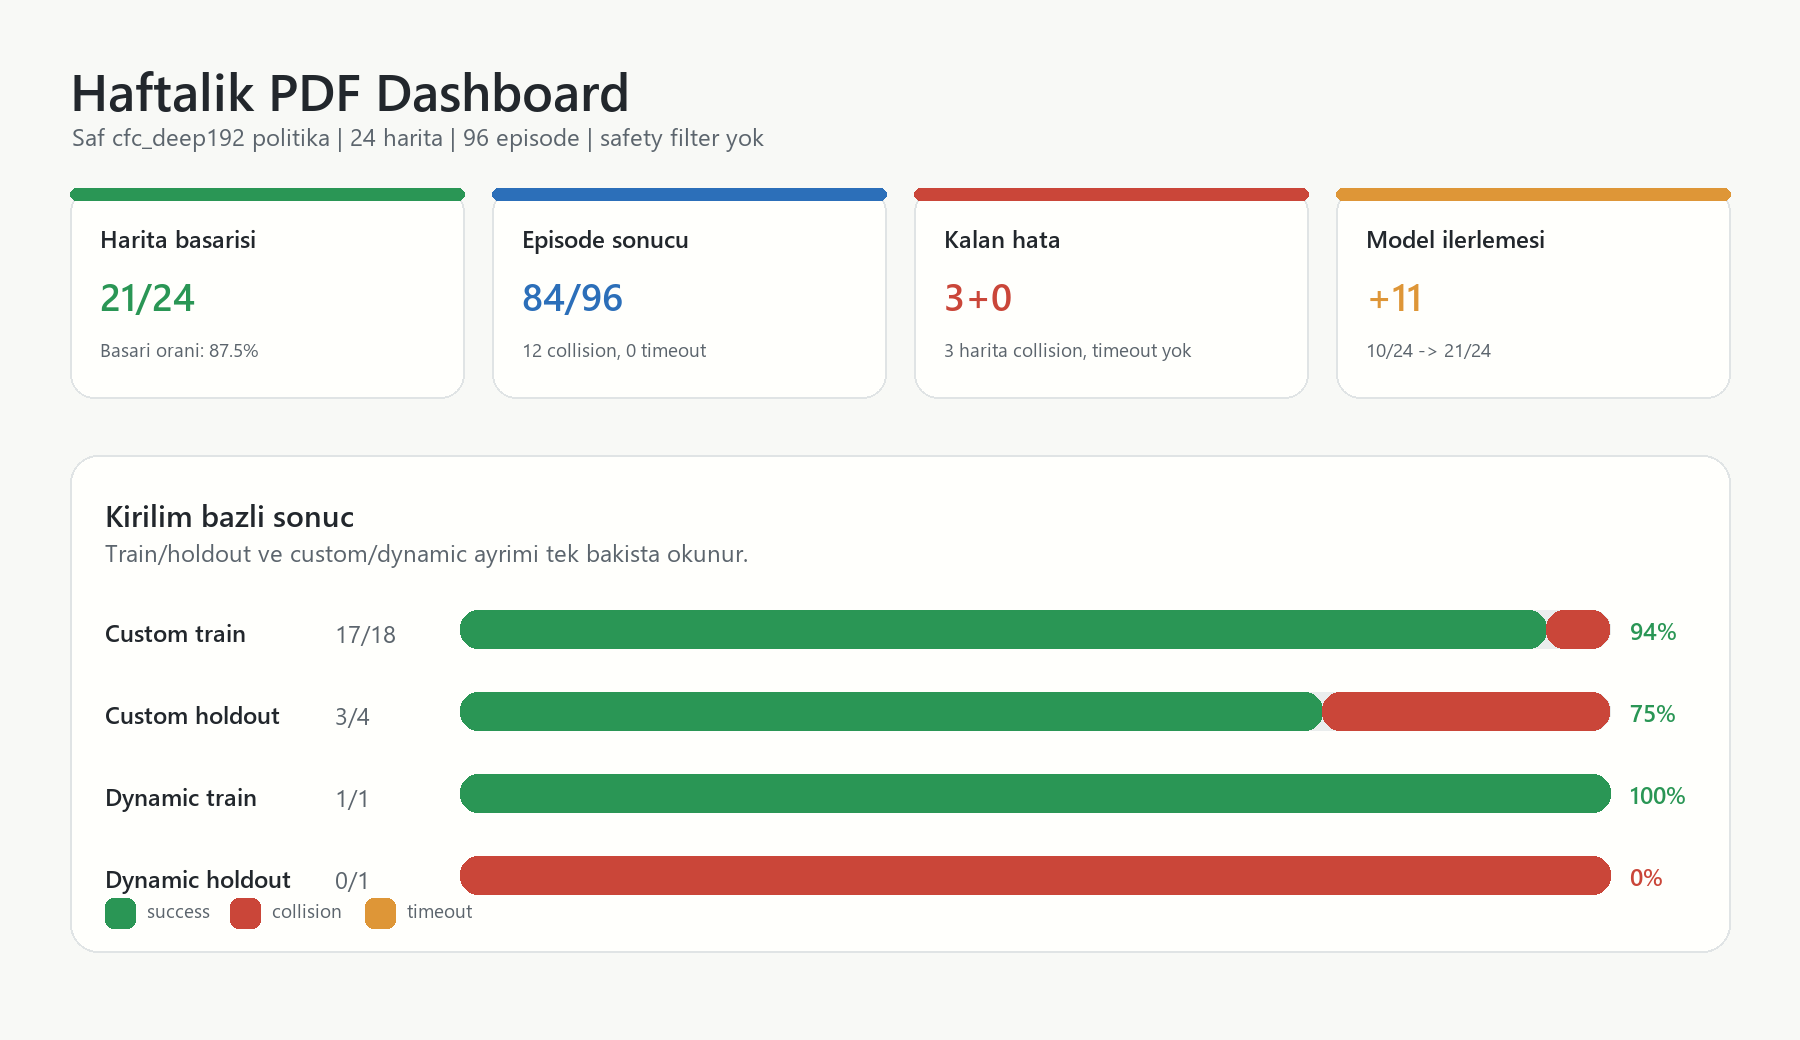
\includegraphics[width=\linewidth]{kpi_dashboard.png}
\caption{Haftalık KPI dashboard'u. Üst kartlar modelin genel sonucunu, alt barlar
train/holdout ve custom/dynamic kırılımını gösterir.}
\label{fig:kpi_dashboard}
\end{figure}

\section{Haftanın Hedefi ve Çıktıları}

Haftanın başlangıç hedefi iki parçadan oluşuyordu: modeli dinamik haritalarda
test etmek ve LNN tabanlı mobil robot navigasyonuyla ilişkili literatürdeki
boşluğu netleştirmek. Çalışma ilerledikçe eski modelin statik haritalarda da
sınırlı genelleme yaptığı görüldü; bu nedenle güvenlik filtresi veya kural
tabanlı kontrol eklemek yerine saf LNN mimarisi daha yüksek kapasiteli hale
getirildi.

\begin{table}[H]
\centering
\caption{Bu hafta tamamlanan ana işler}
\begin{tabularx}{\linewidth}{@{}p{0.27\linewidth}X@{}}
\toprule
\textbf{Başlık} & \textbf{Durum} \\
\midrule
Dinamik harita altyapısı &
\code{map.dynamic\_obstacles} alanı ile hareketli silindir/kutu engelleri
eklendi; çizgisel ve dairesel hareket desteklendi. \\
Görselleştirme &
Rollout PNG/GIF çıktıları hareketli engel izlerini gösterecek şekilde
genişletildi. \\
Yeni model &
\code{cfc\_deep} saf LNN politikası eklendi: \code{Linear+Tanh -> CfC -> CfC}. \\
Colab eğitimi &
\code{cfc\_deep192\_custom22\_dynamic\_dagger2} sıfırdan eğitildi. \\
Tüm harita testi &
22 custom + 2 dinamik haritada, her harita için 4 episode ile değerlendirildi. \\
GitHub güncellemesi &
Kod, config, Colab notebook ve dinamik harita dosyaları GitHub'a aktarıldı. \\
\bottomrule
\end{tabularx}
\end{table}

\section{Mimari Değişikliği}

Önceki yapı tek CfC katmanlıydı. Bu hafta önerilen yeni yapı yine saf LNN
çizgisinde kaldı; modele waypoint takipçisi, safety filter, A* tabanlı runtime
müdahalesi veya kural tabanlı kontrol eklenmedi. Eğitim sırasında öğretmen veri
üretimi için planlama kullanılabilir; ancak değerlendirme anında robotun
aksiyonu sadece politika ağından gelir.

\begin{figure}[H]
\centering
\resizebox{\linewidth}{!}{%
\begin{tikzpicture}[
  node distance=1.15cm,
  block/.style={draw, rounded corners=2pt, align=center, minimum width=2.85cm,
    minimum height=0.9cm, fill=blue!7},
  lnn/.style={draw, rounded corners=2pt, align=center, minimum width=2.85cm,
    minimum height=0.9cm, fill=green!9},
  head/.style={draw, rounded corners=2pt, align=center, minimum width=2.45cm,
    minimum height=0.85cm, fill=orange!12},
  arrow/.style={-Latex, thick}
]
\node[block] (obs) {38-D gözlem\\
\scriptsize hedef uzaklığı/açısı, hız, önceki aksiyon, 32 LiDAR};
\node[block, right=of obs] (enc) {Linear(38,192)\\Tanh};
\node[lnn, right=of enc] (cfc1) {CfC katmanı 1\\\scriptsize $\Delta t=0.08$s};
\node[lnn, right=of cfc1] (cfc2) {CfC katmanı 2\\\scriptsize gizli durum 192};
\node[head, above right=0.65cm and 1.1cm of cfc2] (actor) {Actor\\\scriptsize $[v,\omega] \in [-1,1]^2$};
\node[head, below right=0.65cm and 1.1cm of cfc2] (critic) {Critic\\\scriptsize değer tahmini};
\draw[arrow] (obs) -- (enc);
\draw[arrow] (enc) -- (cfc1);
\draw[arrow] (cfc1) -- (cfc2);
\draw[arrow] (cfc2) -- (actor);
\draw[arrow] (cfc2) -- (critic);
\end{tikzpicture}
}
\caption{Yeni saf Deep CfC/LNN politika mimarisi. Çıkış aksiyonu doğrudan
modelden üretilir; değerlendirme sırasında safety filter veya waypoint
müdahalesi yoktur.}
\label{fig:architecture}
\end{figure}

\begin{table}[H]
\centering
\caption{Yeni eğitim konfigürasyonu}
\begin{tabular}{@{}ll@{}}
\toprule
Parametre & Değer \\
\midrule
Run adı & \code{cfc\_deep192\_custom22\_dynamic\_dagger2} \\
Policy & \code{cfc\_deep} \\
Hidden size & 192 \\
BC epoch & 600 \\
DAgger & 2 iterasyon, her iterasyonda 80 epoch \\
Train haritaları & 18 custom + \code{dynamic\_open\_single} \\
Holdout haritaları & 4 custom + \code{dynamic\_crossing} \\
Episode limiti & 900 adım \\
Değerlendirme & Saf politika, \code{auto-waypoints} kapalı \\
\bottomrule
\end{tabular}
\end{table}

\begin{figure}[H]
\centering
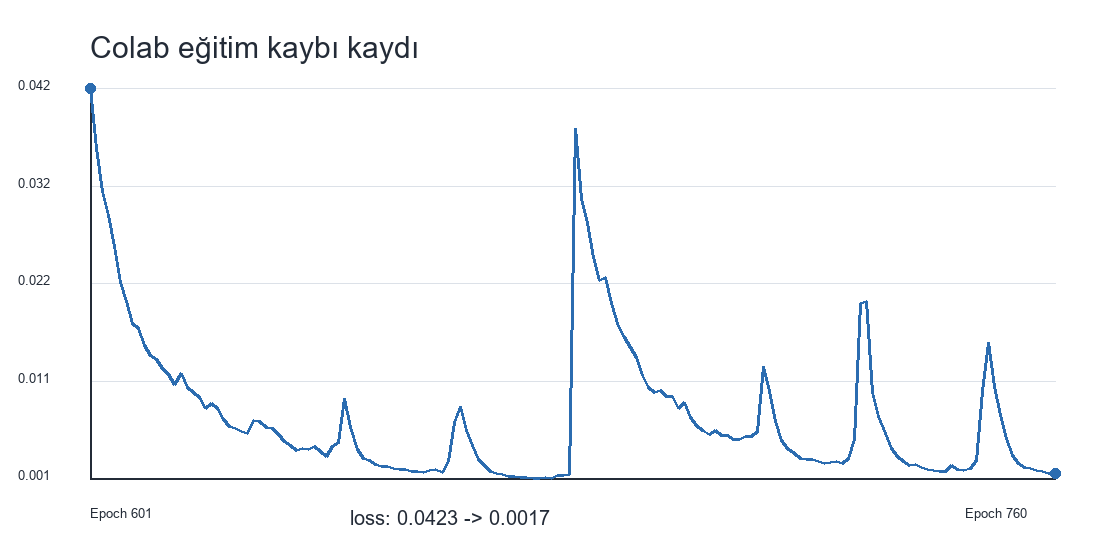
\includegraphics[width=0.82\linewidth]{training_loss.png}
\caption{Colab eğitim kaydı. Dosyadaki son kayıtlar DAgger sonrası epoch 601--760
aralığını göstermektedir; kayıp değeri yaklaşık 0.0423'ten 0.00168'e düşmüştür.}
\label{fig:training_loss}
\end{figure}

\section{Dinamik Harita Altyapısı}

Dinamik harita desteği mevcut gözlem/aksiyon sözleşmesini değiştirmeden eklendi.
Robot hâlâ 38 boyutlu gözlem kullanır ve iki boyutlu aksiyon üretir. Hareketli
engeller LiDAR ışınlarına ve çarpışma kontrolüne dahil edilir. Böylece model
dinamik çevreyi ayrı bir modül üzerinden değil, sensör gözlemi üzerinden
algılamak zorunda kalır.

\begin{table}[H]
\centering
\caption{Yeni dinamik haritalar}
\begin{tabularx}{\linewidth}{@{}p{0.24\linewidth}p{0.18\linewidth}X@{}}
\toprule
Harita & Split & Açıklama \\
\midrule
\code{dynamic\_open\_single} & train &
Açık alanda tek hareketli silindir. Modelin dinamik engelle ilk karşılaşması
için kolay senaryo. \\
\code{dynamic\_crossing} & holdout &
Koridor benzeri statik engeller, hareketli silindir ve hareketli kutu içeren
zor stres testi. Eğitimde kullanılmadı. \\
\bottomrule
\end{tabularx}
\end{table}

\begin{figure}[H]
\centering
\begin{subfigure}{0.48\linewidth}
  \centering
  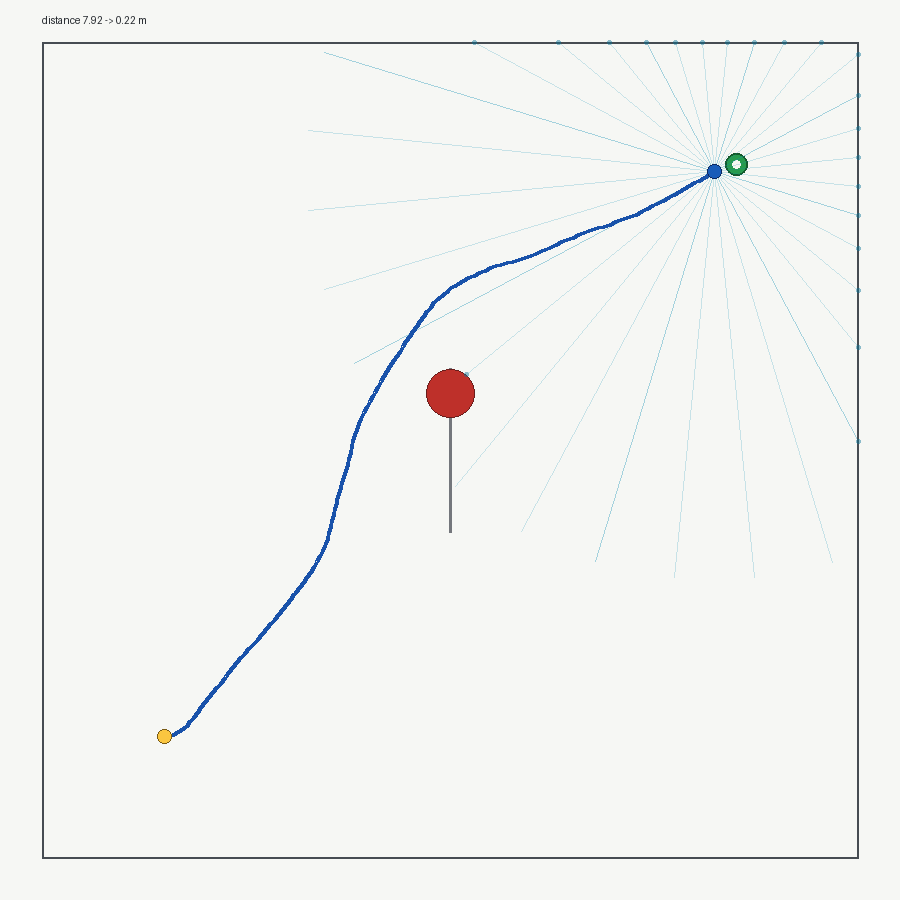
\includegraphics[width=\linewidth]{dynamic_open_single_rollout.png}
  \caption{\code{dynamic\_open\_single}: başarılı rollout}
\end{subfigure}
\hfill
\begin{subfigure}{0.48\linewidth}
  \centering
  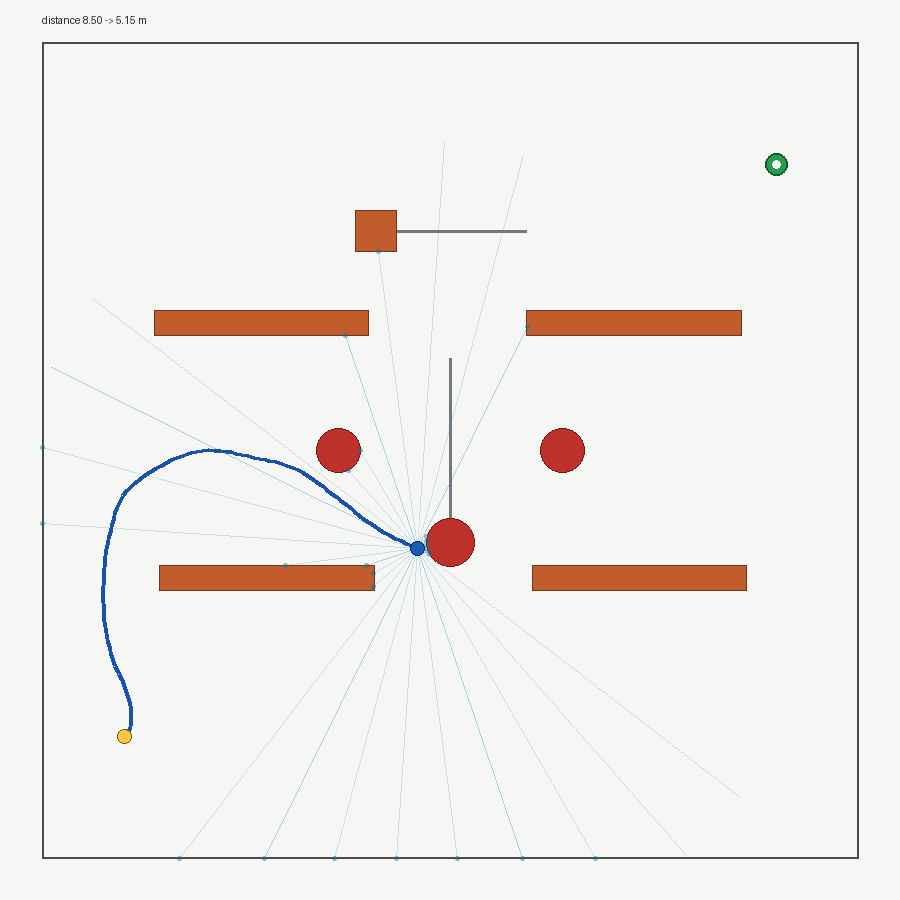
\includegraphics[width=\linewidth]{dynamic_crossing_rollout.png}
  \caption{\code{dynamic\_crossing}: çarpışma}
\end{subfigure}
\caption{Dinamik haritalarda rollout görselleştirmeleri. Hareketli engel izleri
görselleştirmeye dahil edilmiştir.}
\label{fig:dynamic_rollouts}
\end{figure}

\section{Tüm Haritalarda Son Durum}

Yeni checkpoint \code{results/cfc\_deep192\_custom22\_dynamic\_dagger2/latest.pt}
ile tüm haritalarda değerlendirme çalıştırıldı. Her haritada 4 episode koşuldu.
Toplamda 96 episode elde edildi. Başarılı olan 21 haritada 4/4 başarı, başarısız
3 haritada 4/4 çarpışma görüldü. Timeout oranı sıfırdır.

\begin{table}[H]
\centering
\caption{Genel değerlendirme özeti}
\begin{tabular}{@{}lrrrr@{}}
\toprule
Küme & Harita sayısı & Başarı & Çarpışma & Timeout \\
\midrule
Custom train & 18 & 17/18 & 1/18 & 0/18 \\
Custom holdout & 4 & 3/4 & 1/4 & 0/4 \\
Dynamic train & 1 & 1/1 & 0/1 & 0/1 \\
Dynamic holdout & 1 & 0/1 & 1/1 & 0/1 \\
\midrule
Toplam & 24 & 21/24 & 3/24 & 0/24 \\
\bottomrule
\end{tabular}
\end{table}

\begin{figure}[H]
\centering
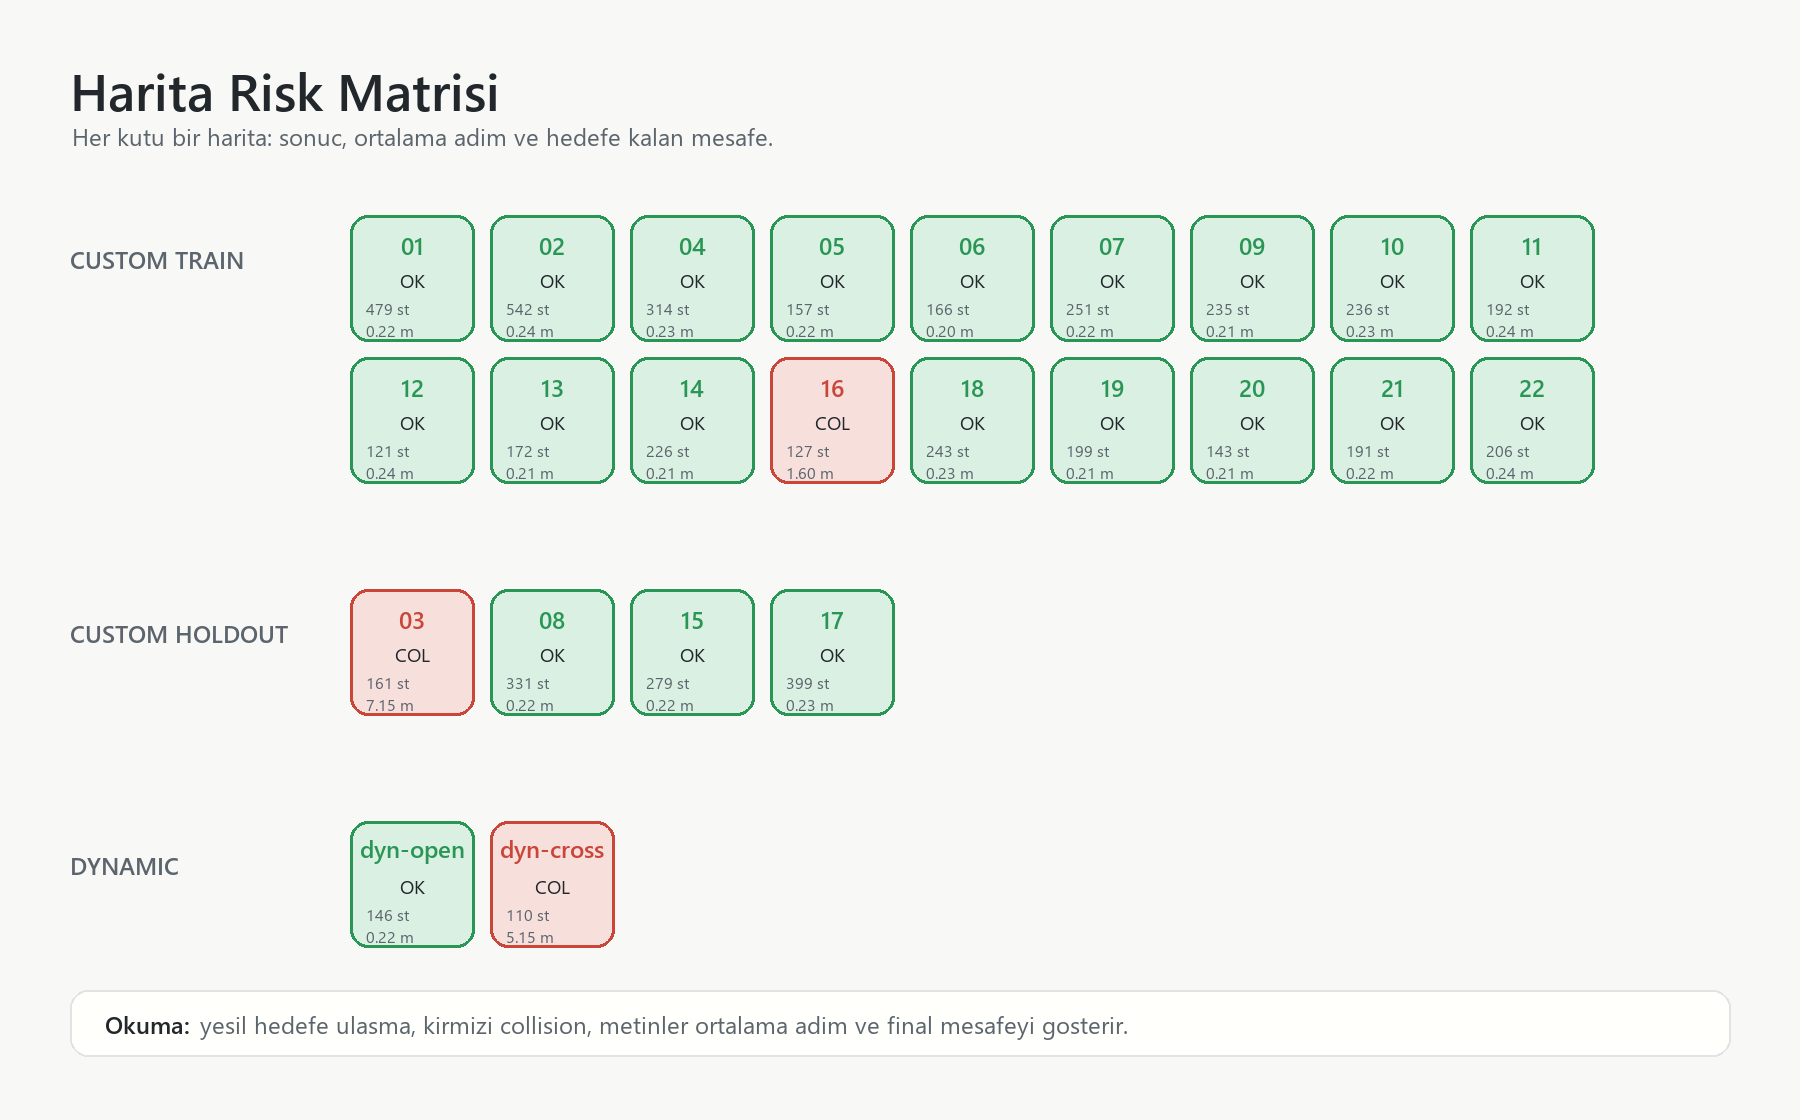
\includegraphics[width=\linewidth]{map_risk_matrix.png}
\caption{Harita risk matrisi. Her kutu bir haritayı temsil eder; renk sonuç
tipini, alt metin ortalama episode adımını ve hedefe kalan mesafeyi gösterir.}
\label{fig:map_risk_matrix}
\end{figure}

\begin{figure}[H]
\centering
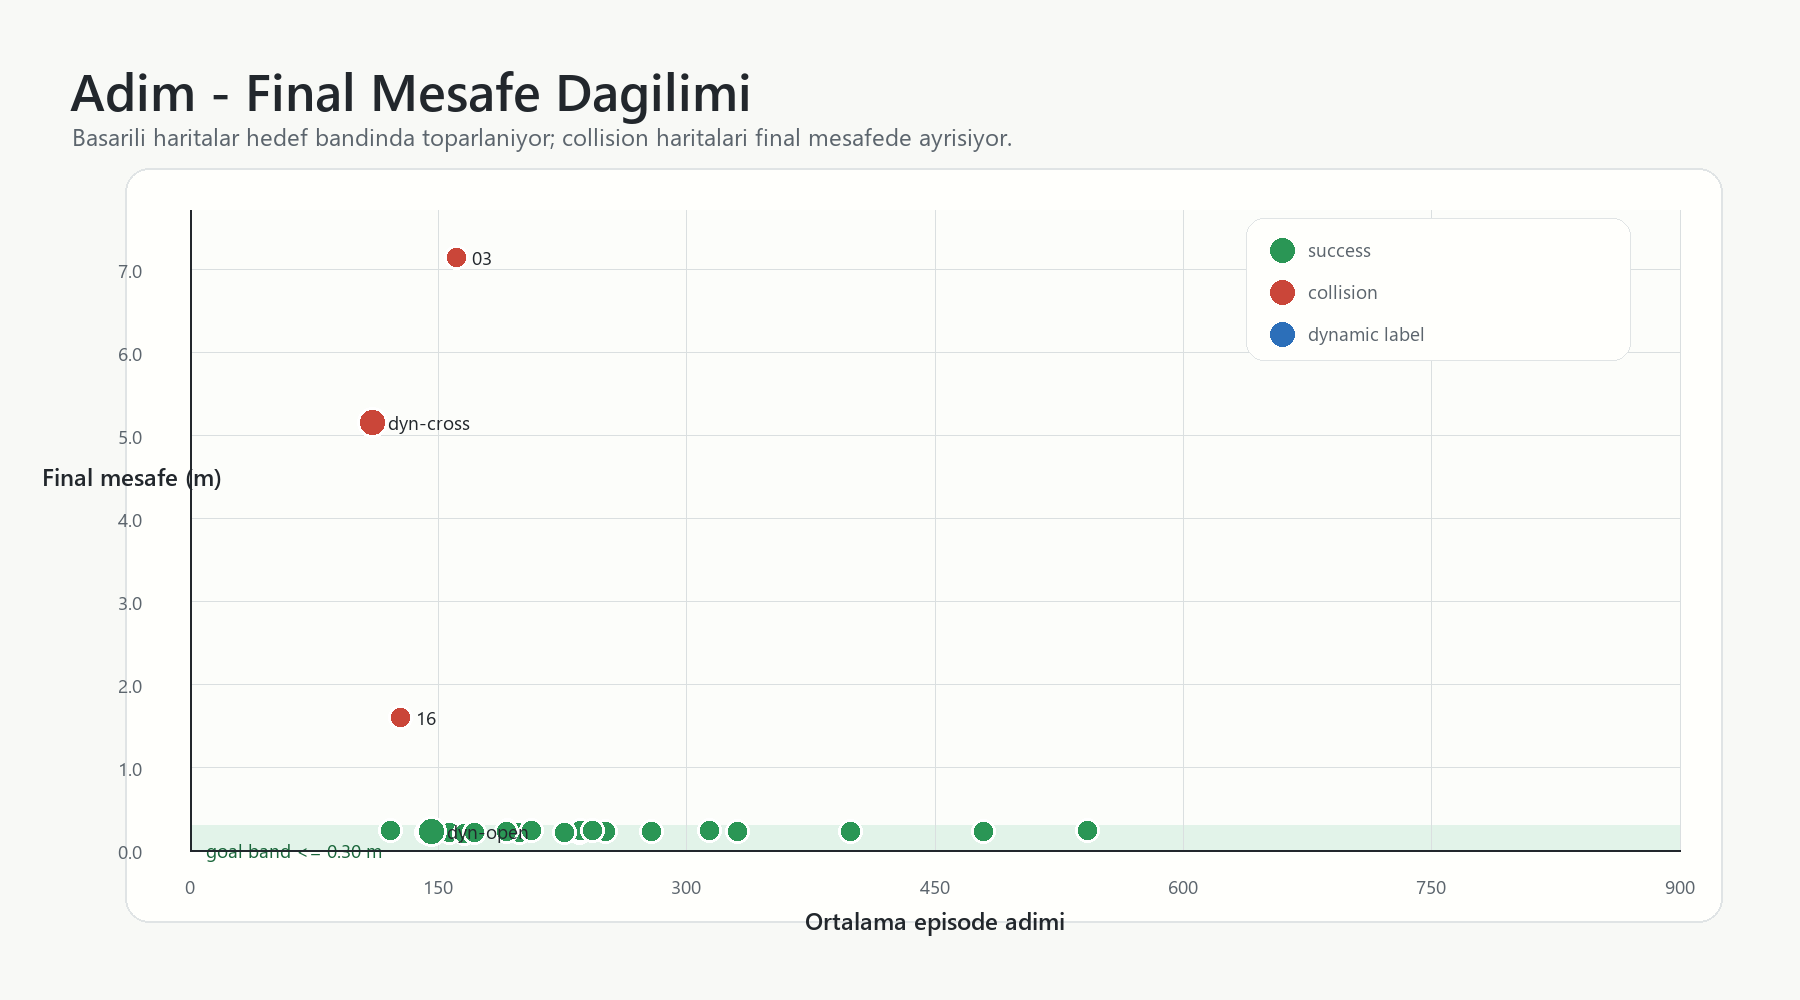
\includegraphics[width=\linewidth]{steps_distance_scatter.png}
\caption{Ortalama episode adımı ile final hedef mesafesi arasındaki dağılım.
Başarılı haritalar hedef bandında kümelenirken üç collision haritası final
mesafede belirgin biçimde ayrışmaktadır.}
\label{fig:steps_distance_scatter}
\end{figure}

\begin{figure}[H]
\centering
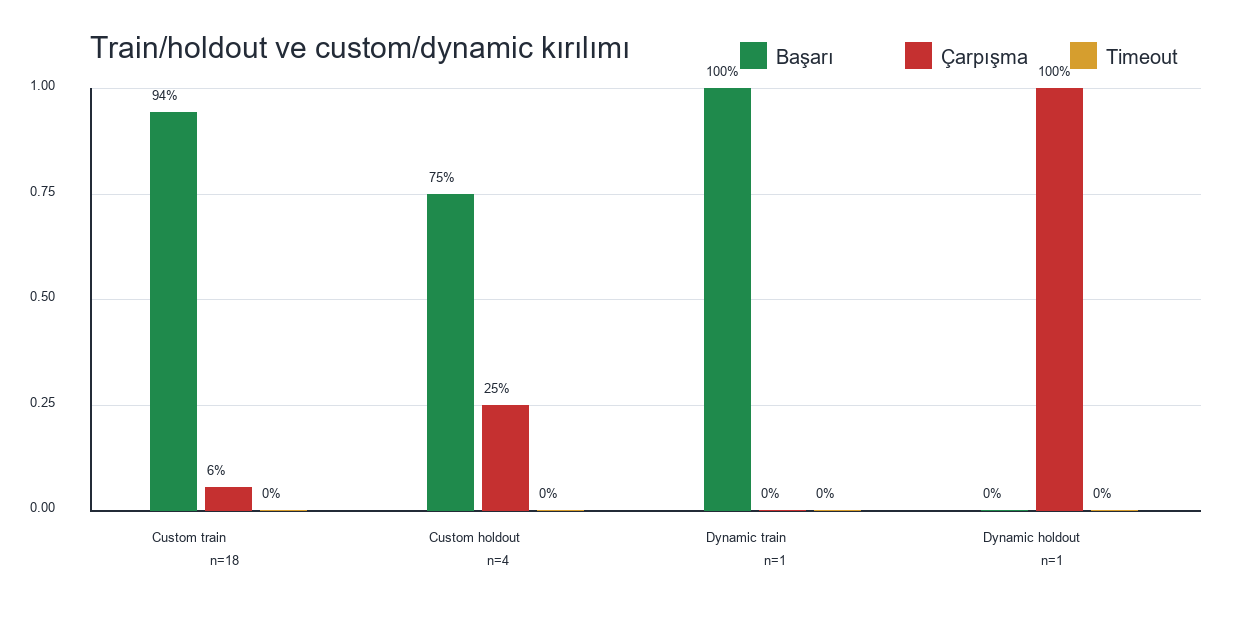
\includegraphics[width=\linewidth]{group_outcomes.png}
\caption{Başarı, çarpışma ve timeout oranlarının train/holdout ve custom/dynamic
kırılımı. Dinamik holdout senaryosu şu an modelin en zayıf noktasıdır.}
\label{fig:group_outcomes}
\end{figure}

\begin{figure}[H]
\centering
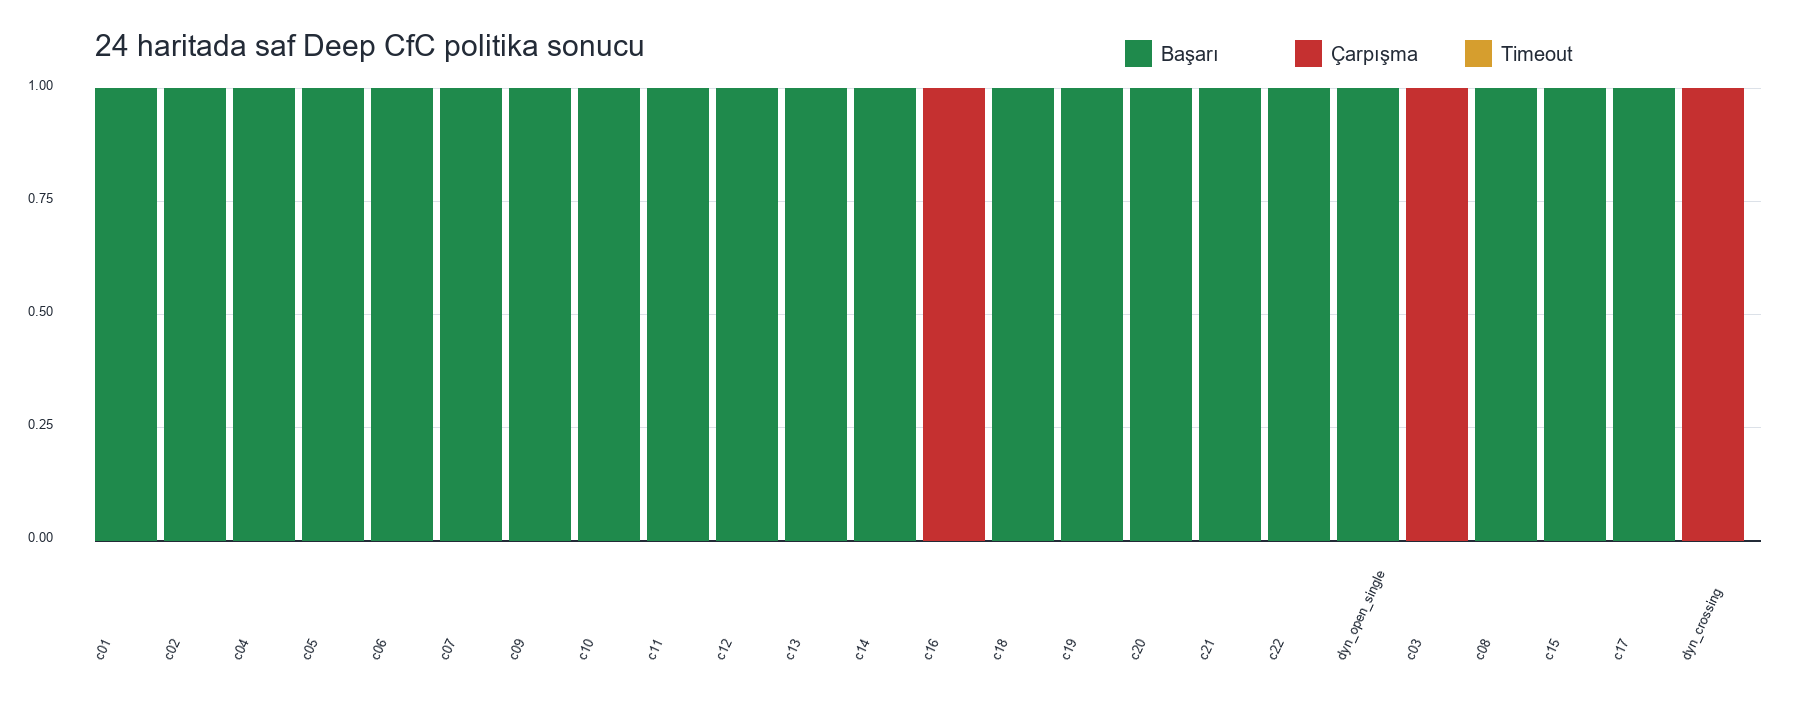
\includegraphics[width=\linewidth]{map_outcomes.png}
\caption{24 haritada harita bazlı sonuçlar. Üç başarısız harita
\code{custom\_map\_16}, \code{custom\_map\_03} ve \code{dynamic\_crossing}
olarak ayrışmaktadır.}
\label{fig:map_outcomes}
\end{figure}

\begin{figure}[H]
\centering
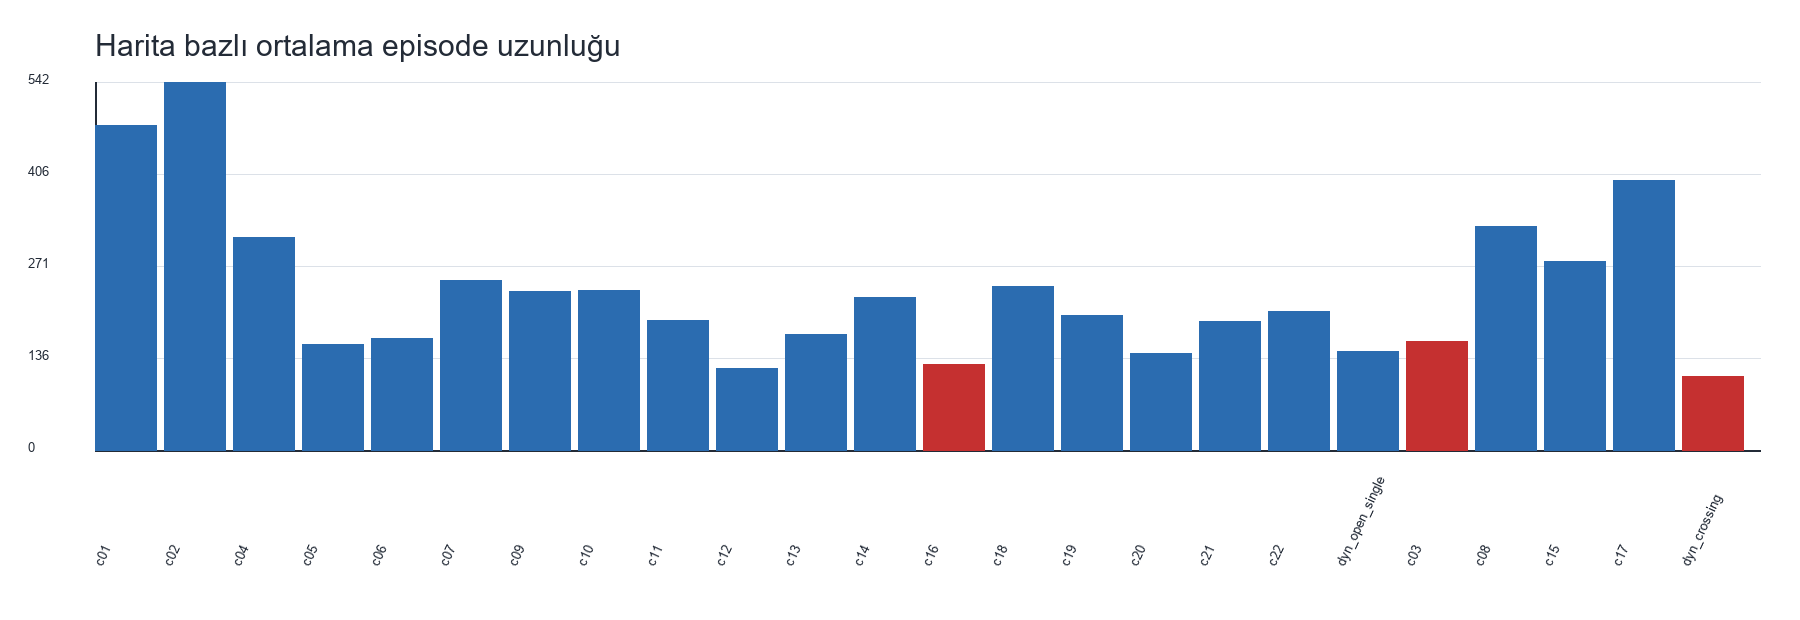
\includegraphics[width=\linewidth]{mean_steps.png}
\caption{Harita bazlı ortalama episode uzunluğu. Başarısız haritalarda episode
çarpışma nedeniyle kısa kesilmektedir; başarılı ama uzun haritalar hedefe
ulaşsa da verimlilik açısından iyileştirilebilir.}
\label{fig:mean_steps}
\end{figure}

\section{Zengin Rollout Görselleştirmeleri}

Aşağıdaki grid tüm 24 haritanın rollout görüntülerini aynı sayfada gösterir.
Yeşil başlıklar başarılı haritaları, kırmızı başlıklar çarpışmayla sonuçlanan
haritaları temsil eder.

\begin{figure}[H]
\centering
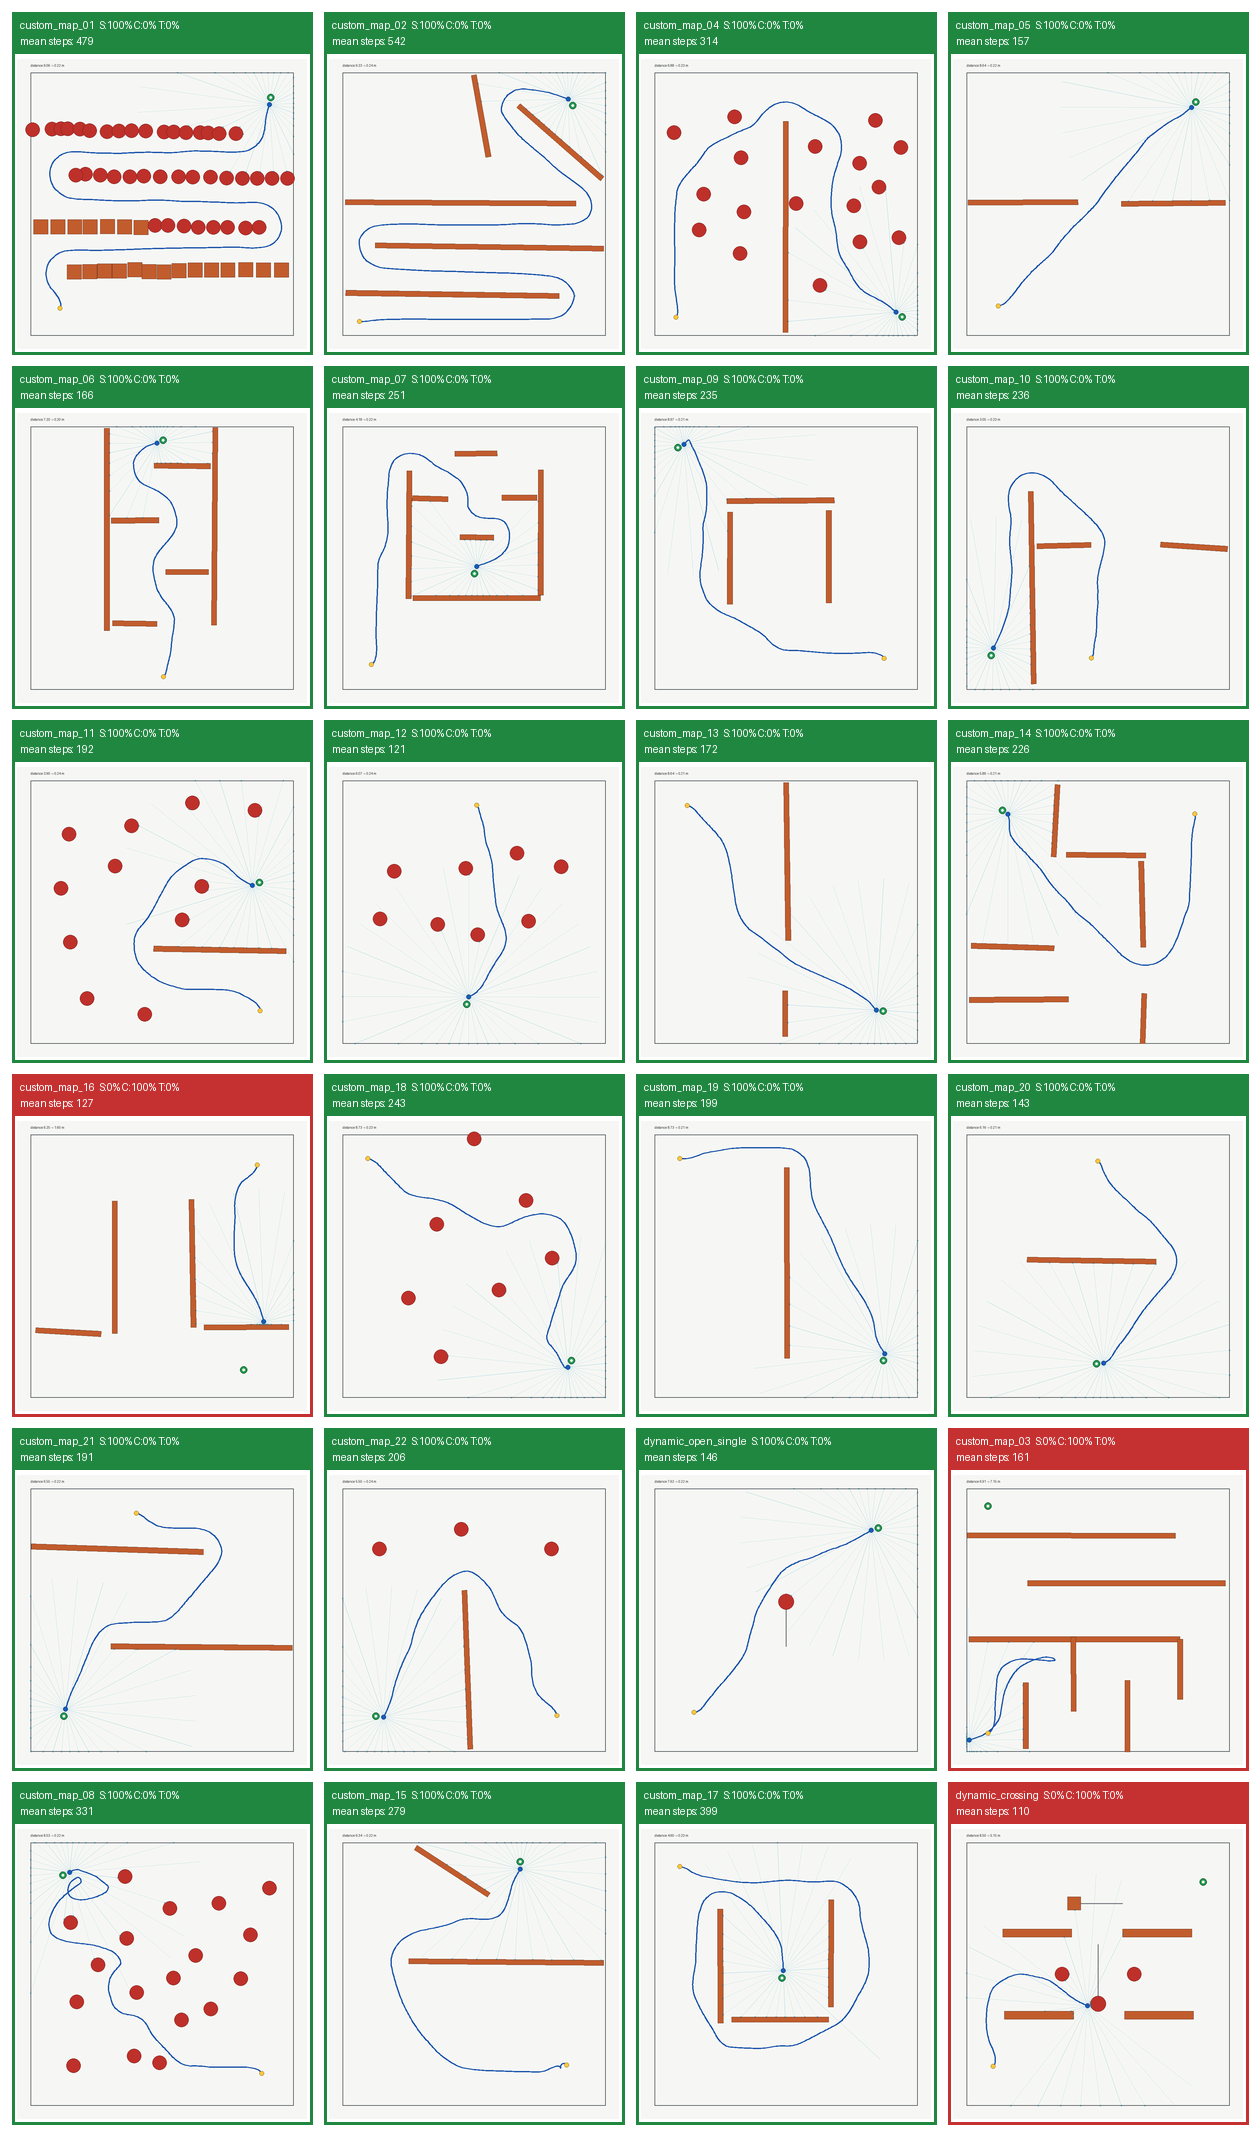
\includegraphics[height=0.83\textheight,keepaspectratio]{all24_rollout_grid.png}
\caption{Tüm 24 harita için rollout grid'i.}
\label{fig:all_rollouts}
\end{figure}

\begin{figure}[H]
\centering
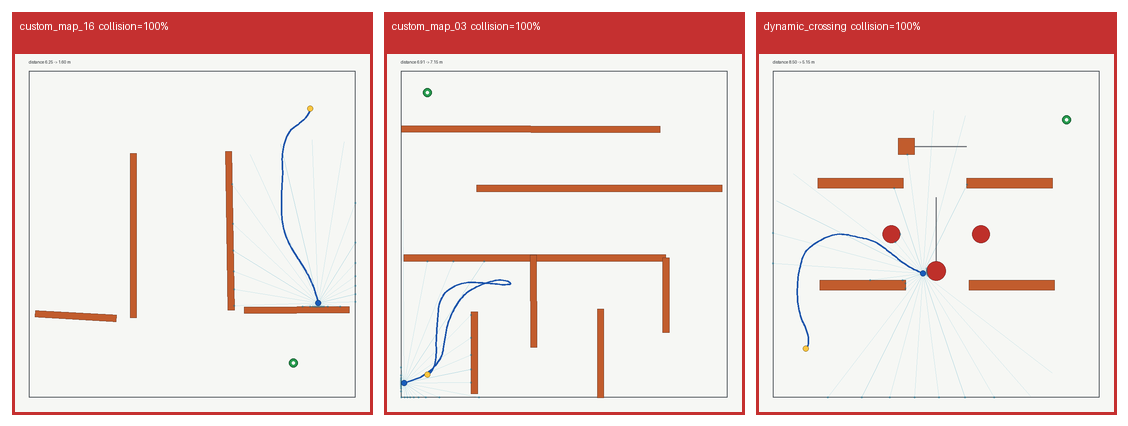
\includegraphics[width=\linewidth]{failed_rollouts_grid.png}
\caption{Başarısız üç haritanın yakın görünümü. Hata modu timeout değil,
doğrudan çarpışmadır.}
\label{fig:failed_rollouts}
\end{figure}

\begin{figure}[H]
\centering
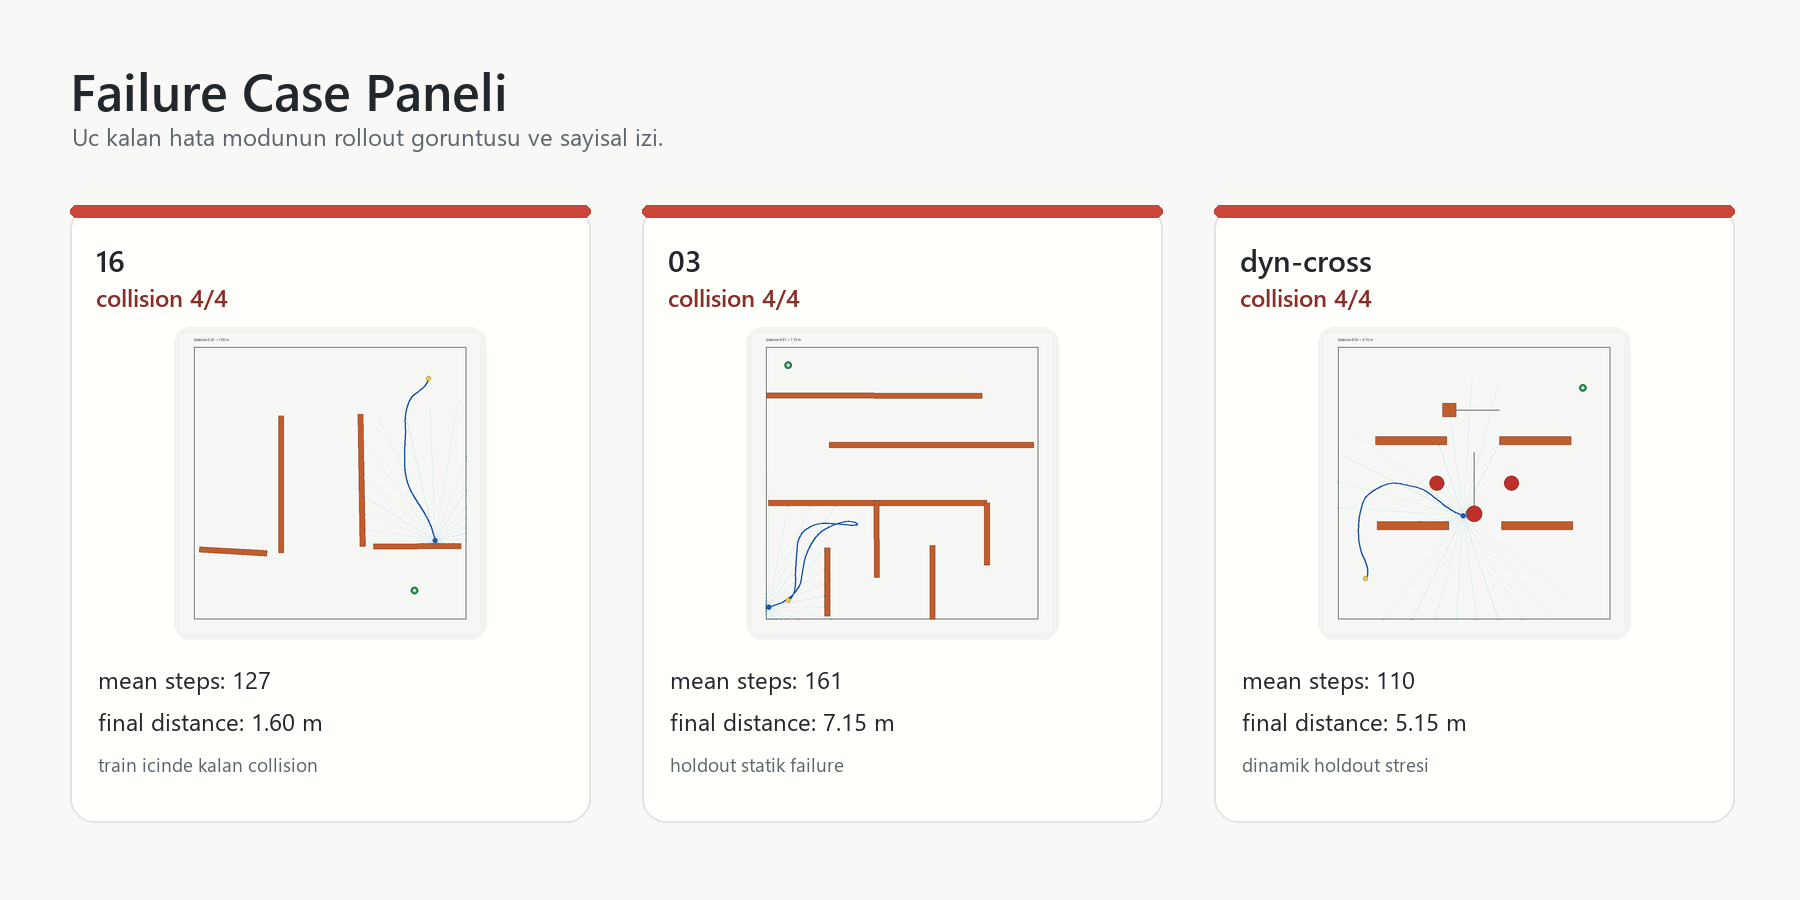
\includegraphics[width=\linewidth]{failure_cases_panel.png}
\caption{Kalan üç failure case için rollout görüntüsü ve sayısal özet. Bu panel,
sonraki hafta çıkarılacak LiDAR/aksiyon zaman serisi analizine giriş noktasıdır.}
\label{fig:failure_cases_panel}
\end{figure}

\section{Önceki Modele Göre İlerleme}

Önceki \code{cfc\_radius010\_custom22\_dagger2} modeli aynı 24 haritalık
değerlendirmede 10/24 başarı üretmişti. Yeni \code{cfc\_deep192} modeliyle bu
değer 21/24'e çıktı. En önemli fark, modelin hedefe yönelme ve dar olmayan
statik haritalarda kararlı ilerleme davranışının belirgin şekilde iyileşmesidir.

\begin{table}[H]
\centering
\caption{Model ilerleme özeti}
\small
\begin{tabularx}{\linewidth}{@{}p{0.28\linewidth}ccX@{}}
\toprule
Model & Harita & Başarı & Not \\
\midrule
\begin{tabular}{@{}l@{}}\code{cfc\_radius010}\\\code{custom22\_dagger2}\end{tabular} & 24 & 10/24 &
Tek katmanlı CfC; dinamik kolay harita başarılı, birçok custom haritada
timeout/başarısızlık. \\
\begin{tabular}{@{}l@{}}\code{cfc\_deep192}\\\code{custom22\_dynamic}\\\code{dagger2}\end{tabular} & 24 & 21/24 &
İki katmanlı saf CfC; timeout yok, kalan hata modu çarpışma. \\
\bottomrule
\end{tabularx}
\end{table}

\begin{figure}[H]
\centering
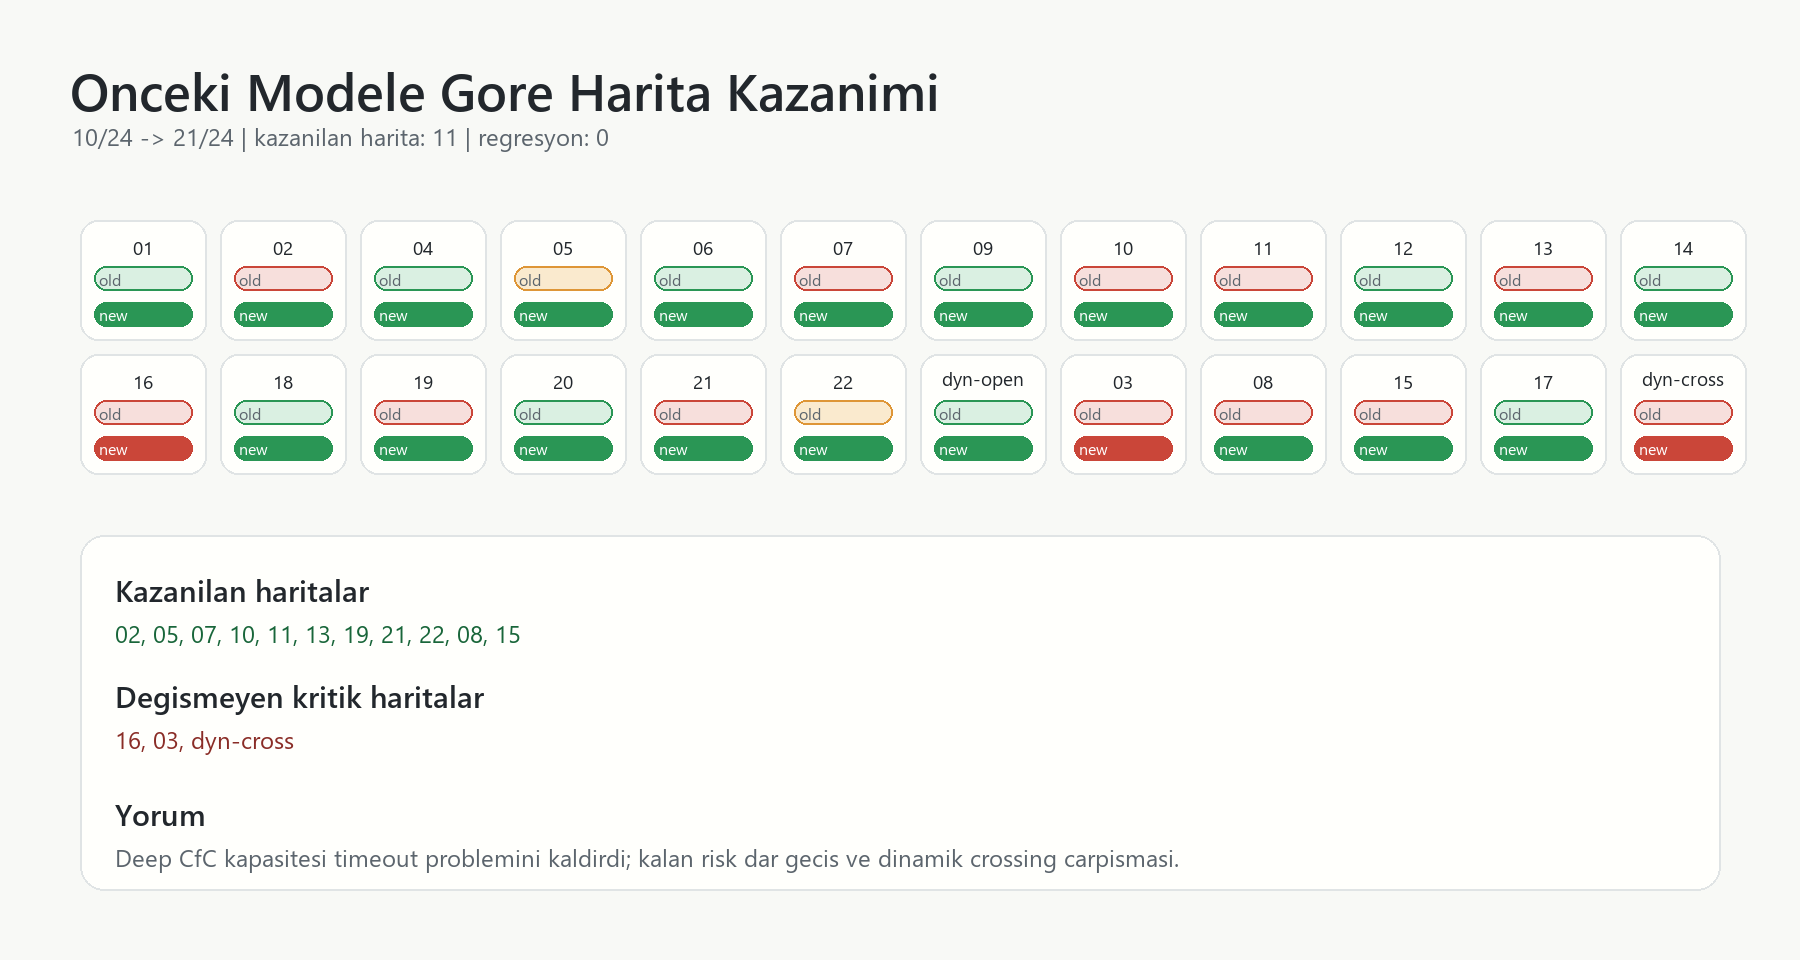
\includegraphics[width=\linewidth]{model_delta_grid.png}
\caption{Eski tek katmanlı CfC ile yeni Deep CfC modelinin harita bazlı
karşılaştırması. Yeşil alt şeritler yeni modelin kazandığı haritaları,
kırmızı alt şeritler hâlâ çözülmeyen failure case'leri gösterir.}
\label{fig:model_delta_grid}
\end{figure}

\section{Literatür Notu ve Konumlandırma}

Literatür taramasında doğrudan ``MuJoCo + diferansiyel sürüşlü mobil robot +
LiDAR + LNN/CfC + dinamik engel'' kombinasyonuna birebir karşılık gelen bir
çalışma bulunmadı. En yakın çalışmalar LNN/LTC/CfC'nin görsel drone navigasyonu,
OOD genelleme ve sürekli zamanlı kontrol üzerindeki başarılarını gösteriyor.
Bu nedenle proje için savunulabilir araştırma boşluğu şudur: düşük boyutlu
LiDAR gözlemiyle çalışan bir kara robotunda saf CfC/LNN politikasının statik ve
dinamik harita kaymalarında sistematik değerlendirilmesi.

\section{Kalan Sorunlar ve Sonraki Hafta Planı}

Mevcut sonuçlar saf LNN yaklaşımının güçlü biçimde ilerlediğini gösteriyor;
ancak çarpışma problemi üç haritada açık biçimde devam ediyor. Özellikle
\code{dynamic\_crossing} eğitimde görülmediği için dinamik holdout genellemesi
henüz yeterli değil.

\begin{enumerate}
  \item \textbf{Başarısız harita analizi:} \code{custom\_map\_03},
  \code{custom\_map\_16} ve \code{dynamic\_crossing} için çarpışma anındaki
  LiDAR profilleri ve aksiyon dizileri çıkarılacak.
  \item \textbf{Saf LNN içinde iyileştirme:} Safety filter eklemeden,
  dinamik engel varyasyonları ve başarısız harita benzeri eğitim örnekleri
  artırılacak.
  \item \textbf{Holdout disiplini:} \code{dynamic\_crossing} bir süre daha
  holdout olarak korunacak; benzer ama aynı olmayan yeni dinamik train haritaları
  üretilecek.
  \item \textbf{Rapor metrikleri:} Başarı/çarpışma oranına ek olarak minimum
  LiDAR mesafesi, hedefe kalan mesafe ve aksiyon pürüzlülüğü raporlanacak.
\end{enumerate}

\section{Kısa Sonuç}

Bu haftanın teknik sonucu nettir: dinamik harita altyapısı tamamlandı, saf
Deep CfC/LNN mimarisi projeye eklendi ve Colab eğitimi sonrası tüm harita
başarısı 10/24'ten 21/24'e yükseldi. Model artık timeout yerine çoğu haritada
hedefe ulaşabilmektedir. Kalan problem, belirli dar/geçiş senaryolarında
çarpışma davranışıdır. Sonraki çalışma, mimariye kural tabanlı güvenlik katmanı
eklemeden bu çarpışma modunu eğitim verisi ve saf LNN kapasitesi içinde
azaltmaya odaklanmalıdır.

\end{document}
